% 2003 年全国旧课程文科第 22 题：矩形动点示意图
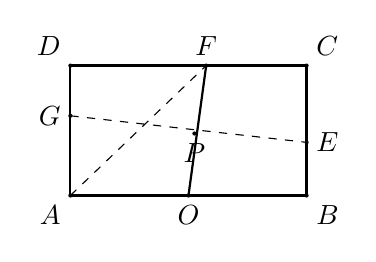
\begin{tikzpicture}[>=stealth,scale=0.75]
  \coordinate (A) at (0,0); \coordinate (B) at (4,0);
  \coordinate (C) at (4,2.2); \coordinate (D) at (0,2.2);
  \coordinate (E) at (4,0.9); \coordinate (F) at (2.3,2.2);
  \coordinate (G) at (0,1.35); \coordinate (P) at (2.1,1.05);
  \coordinate (O) at (2,0);
  \draw[thick] (A)--(B)--(C)--(D)--cycle;
  \draw[dashed] (G)--(E) (A)--(F);
  \draw[thick] (O)--(F);
  \fill (A) circle (1pt) node[below left] {$A$};
  \fill (B) circle (1pt) node[below right] {$B$};
  \fill (C) circle (1pt) node[above right] {$C$};
  \fill (D) circle (1pt) node[above left] {$D$};
  \fill (E) circle (1pt) node[right] {$E$};
  \fill (F) circle (1pt) node[above] {$F$};
  \fill (G) circle (1pt) node[left] {$G$};
  \fill (P) circle (1pt) node[below] {$P$};
  \fill (O) circle (1pt) node[below] {$O$};
\end{tikzpicture}
